\section{Convolutional Neural Network}
Die Evaluation des Suchalgorithmus hat einen klaren Sieger ergeben. Das Convolutional\footnote{Convolutional ist Englisch und heisst auf Deutsch Faltung} Neural Network (hier weiter als Convnet bezeichnet) liefert mit Abstand die besten Resultate innerhalb unserer Test Bounding Box in Rapperswil.

\subsection{Geschichte}
Bis noch vor einigen Jahren wurden neuronale Netze zur Bilderkennung grösstenteils ignoriert\footnote{\url{http://karpathy.github.io/2015/10/25/selfie/}}. Das Convnet selbst wurde schon 1980 von einem Japaner namens Fukushima erfunden, jedoch erhielt es keine grössere Beachtung. Hauptgrund dafür war der Rechenhunger für das Training des Netzes. Gedreht hat sich das Ganze erst als 2012 genügend Rechenleistung mithilfe von Grafikkarten zur Verfügung stand. Ab diesem Zeitpunkt erzielte diese wieder gefundene Technik Bestleistungen in vielen Bereichen der Bilderkennung. Bis heute ist das Convnet die präziseste Technik zur Erkennung von Gegenständen in Fotos.

\subsection{Funktionsweise}
Ein künstliches neuronales Netz besteht aus einer grossen Anzahl von simulierten Neuronen. Mit verschiedenen Techniken aus der Statistik und  Mathematik kann so ein Input auf einen Output gemappt werden. In unserem Fall wollen wir ein Bild auf eine der Kategorien Crosswalk oder Non-Crosswalk mappen. Dies wird in der Fachliteratur auch Klassifikation von Bildern genannt.

Wie der Name schon sagt, besteht das Convolutional Neuronale Netz aus vielen verschiedenen Faltungsfilter. Ein Faltungsfilter transformiert Bild so, dass es ein spezifisches Muster auf dem Bild markiert wird. Ein gutes Beispiel für einen Filter ist die Technik der Kantendetektion\footnote{\url{https://de.wikipedia.org/wiki/Kantendetektion}}. Die Kantendetektion markiert nur die Kanten auf dem Bild und ignoriert den restlichen Inhalt.

\begin{figure}[H]
	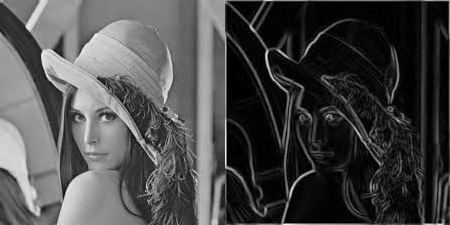
\includegraphics[width=\textwidth]{images/kantendetektion.jpg}
	\caption{Beispiel einer Kantendetektion}
\end{figure}

Ein Convolutional Neuronales Netz lernt nun selbst, welchen Faltungsfilter er anwendet, um das Problem möglichst gut zu lösen. Die extrahierten Muster dienen als Features und werden nun von einem einfachen Neuronalen Netz klassifiziert. Die Ausgabe besteht nun aus aus zwei Werten zwischen 0 und 1. Sie stellen die Wahrscheinlichkeiten der entsprechenden Klasse dar.

\subsection{Keras}
Das Projekt Keras\footnote{\url{https://github.com/fchollet/keras}} stellt eine einfache Library zum Entwerfen und Trainieren von Neuronalen Netzen zur Verfügung. Es bietet modulare Funktionen für Convolutional Neuronale Netzwerke und Rekurrente Netzwerke an. Mithilfe eines Flags kann das Training einfach auf die Grafikkarte ausgelagert werden, was bei solchen Algorithmen unerlässlich ist.